\chapter{Convolutional Neural Network (CNN/ ConvNet) \cite{gfg-convolutional-neural-network-cnn-in-machine-learning}}\label{Convolutional Neural Network}

\begin{enumerate}
    \item Convolutional Neural Networks, or CNNs, are a specialized class of neural networks designed to effectively process grid-like data, such as images.

    \item A Convolutional Neural Network (CNN) is a type of deep learning algorithm that is particularly well-suited for image recognition and processing tasks.
\end{enumerate}


\section{Components}
\subsection{Kernel/ Filter}


\section{Layers}
\subsection{Convolutional Layer}

SEE: \fullref{nn: Convolution Layer}


\subsection{Pooling Layer}

SEE: \fullref{nn: Pooling Layer}


\subsection{Fully Connected Layer/ Dense Layer}
SEE: \fullref{nn: Linear Layer/ Dense Layer}



\section{General Network Design \cite{gfg-convolutional-neural-network-cnn-in-machine-learning}}\label{cnn: General Network Design}

\begin{figure}[h]
    \centering
    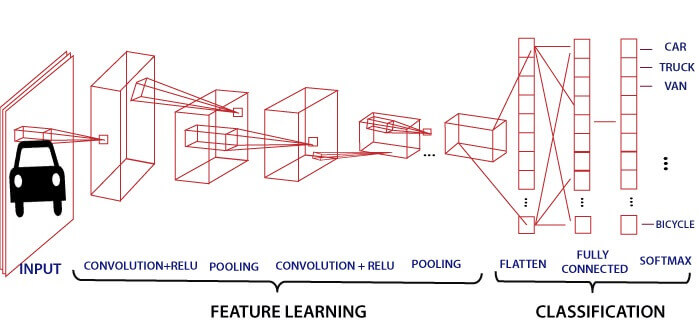
\includegraphics[width=\linewidth, height=5cm, keepaspectratio]{Pictures/convolutional-neural-network/convolutional-neural-network.jpg}
    \caption{CNN: General Network Design}
\end{figure}

\begin{enumerate}
    \item The construction of a convolutional neural network is a multi-layered feed-forward neural network, made by assembling many unseen layers on top of each other in a particular order.

    \item It is the sequential design that give permission to CNN to learn hierarchical attributes.
    
    \item In CNN, some of them followed by grouping layers and hidden layers are typically convolutional layers followed by activation layers.
    
    \item The pre-processing needed in a ConvNet is kindred to that of the related pattern of neurons in the human brain and was motivated by the organization of the \textbf{Visual Cortex}.
\end{enumerate}


\section{Formula}
\[
   \displaystyle n_{out} = \left[ \dfrac{n_{in} + 2p - k}{s} \right] + 1
   \hfill
   \text{ (sometimes $k=f$)}
\]

\begin{table}[H]
    \begin{minipage}[t]{0.5\linewidth}
        \begin{alternateColorTable}
        \begin{table}[H]
            \begin{tabular}{|l l|}
                \hline
                $n_{in}$ & number of input features \\
                $n_{out}$ & number of output features \\
                $k$ & kernel size $k\times k$ / $\dParenBrac{k, k}$ \\
                $p$ & padding size \\
                $s$ & stride size $s\times s$ / $\dParenBrac{s, s}$ \\
                \hline
            \end{tabular}
        \end{table}
        \end{alternateColorTable}
    \end{minipage}
    \hfill
    \begin{minipage}[t]{0.5\linewidth}
        \begin{alternateColorTable}
        \renewcommand{\arraystretch}{1.3}
        \begin{table}[H]
            \begin{tabular}{|l|l|}
                \hline
                \tableHeaderRow
                \multicolumn{2}{|c|}{Padding Types}\\ \hline
                \tableHeaderRow
                \textbf{Type} & $\mathbf{p}$ \textbf{value} \\ \hline
                Valid & 0 \\
                Same & \( \displaystyle p = \dfrac{k - 1}{2} \) \\
                \hline
            \end{tabular}
        \end{table}
        \renewcommand{\arraystretch}{1}
        \end{alternateColorTable}
    \end{minipage}
\end{table}







